\section{Grundlagen Drehfeldmaschinen}
    \subsubsection{Stern- (Y) / Dreieckschaltung ($\Delta$)}
        \renewcommand{\arraystretch}{2}
        \begin{tabular}{| p{4.5cm} | l | l |}
            \hline
            &
            Sternschaltung (Y) &
            Dreieckschaltung ($\Delta$) \\
            \hline
            \vspace{0.2cm} &
            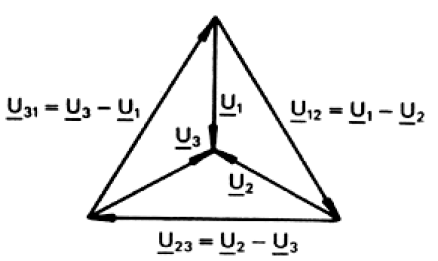
\includegraphics[width=5cm]{images/Sternspannung.png} &
            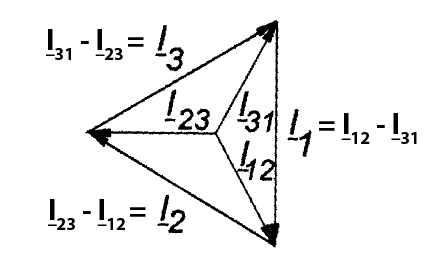
\includegraphics[width=5cm]{images/Dreieckstrom.png} \\
            \hline
            Verkettete Spannung &
            $U = U_{Str} \cdot \sqrt{3}$ \hspace{0.2cm} $\underline{U} = \underline{U}_{Str} \cdot \sqrt{3} \cdot e^{j 30^\circ}$ &
            $U = U_{Str}$ \hspace{0.2cm} $\underline{U} = \underline{U}_{Str}$ \\
            \hline
            Aussenleiterströme &
            $I = I_{Str}$ \hspace{0.2cm} $\underline{I} = \underline{I}_{Str}$ &
            $I = I_{Str} \cdot \sqrt{3} $ \hspace{0.2cm} $\underline{I} = \underline{I}_{Str} \cdot \sqrt{3} \cdot e^{-j 30^\circ} $ \\
            \hline
            Gesamt-Scheinleistung &
            $S = 3 \cdot S_{Str} =\sqrt{3} \cdot U \cdot I $ \hspace{0.2cm} in $[VA]$ &
            $S = 3 \cdot S_{Str} = \sqrt{3} \cdot U \cdot I$ \hspace{0.2cm} in $[VA]$ \\
            \hline
            Scheinleistung pro Strang &
            \multicolumn{2}{l|}{\hspace{3cm} $S_{Str} = U_{Str} \cdot I_{Str}$ \hspace{0.2cm} in $[VA]$} \\
            \hline
            Wirkleistung &
            \multicolumn{2}{l|}{\hspace{3cm} $P = S \cdot \cos\varphi = \sqrt{3} \cdot U \cdot I \cdot \cos\varphi$ \hspace{0.2cm} in $[W]$} \\
            \hline
            Blindleistung &
            \multicolumn{2}{l|}{\hspace{3cm} $Q = S \cdot \sin\varphi = \sqrt{3} \cdot U \cdot I \cdot \sin\varphi$ \hspace{0.2cm} in $[var]$} \\
            \hline
        \end{tabular}
        \renewcommand{\arraystretch}{1.5}

    \subsubsection{Stern-Dreieck-Umwandlung}
        \begin{minipage}[lt]{7.5 cm}
            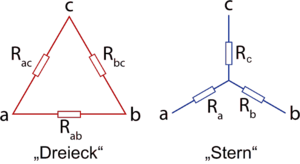
\includegraphics[width=6cm]{images/stern-dreieck.png}
        \end{minipage}
        \begin{minipage}[rt]{9.35 cm} %BASTEL!!
            \renewcommand{\arraystretch}{2}
            \begin{tabular}{ll}
                Umwandlung $\triangle \rightarrow Y$: &
                $Z_{c} = \dfrac{Z_{ac} Z_{bc}}{Z_{ab}+Z_{bc}+Z_{ac}}$ \\
                & $I_{ab} = \frac{I_a \cdot Z_a - I_b \cdot Z_b}{Z_{ab}}$ \\
\                Umwandlung $Y \rightarrow \triangle$: &
                $Y_{ac}=\dfrac{Y_{a} Y_{c}}{Y_{a}+Y_{b}+Y_{c}}$ \\
                Bei gleichen Widerständen: &
                $R_Y = \frac{R_\triangle}{3}$ \\
                Bei gleichen Kapazitäten: &
                $C_Y = C_\triangle \cdot 3 $ \\
                Bei gleichen Induktivitäten: &
                $L_Y = \frac{L_\triangle}{3}$
            \end{tabular}
            \renewcommand{\arraystretch}{1.5}
        \end{minipage}
       